\documentclass[8.5pt]{beamer}

\usetheme{Warsaw}
\definecolor{primary}{RGB}{219, 4, 85}
\usecolortheme[named=primary]{structure}
\setbeamertemplate{headline}{}
\usefonttheme{serif} 

\usepackage[utf8]{inputenc}

\usepackage[T1]{fontenc}
\usepackage[font=small, labelfont=bf]{caption}
 
\title[]{
Blockchain and Geo-spatial Information Systems 
\small{
Blockchain y los Sistemas de Información Geoespacial
}
}
\author{William Condori Quispe}
\institute{Unversidad Nacional Amazónica de Madre de Dios}
\date{2022}

\begin{document}

\maketitle

\section{Introduction}
\section{Artificial intelligence}

\begin{frame}
\frametitle{Deep Learning}
This is some text in the first frame. This is some text in the first frame. This is some text in the first frame.
\end{frame}

\begin{frame}
\frametitle{Convolutional Neural Networks}
\begin{figure}
    \centering
    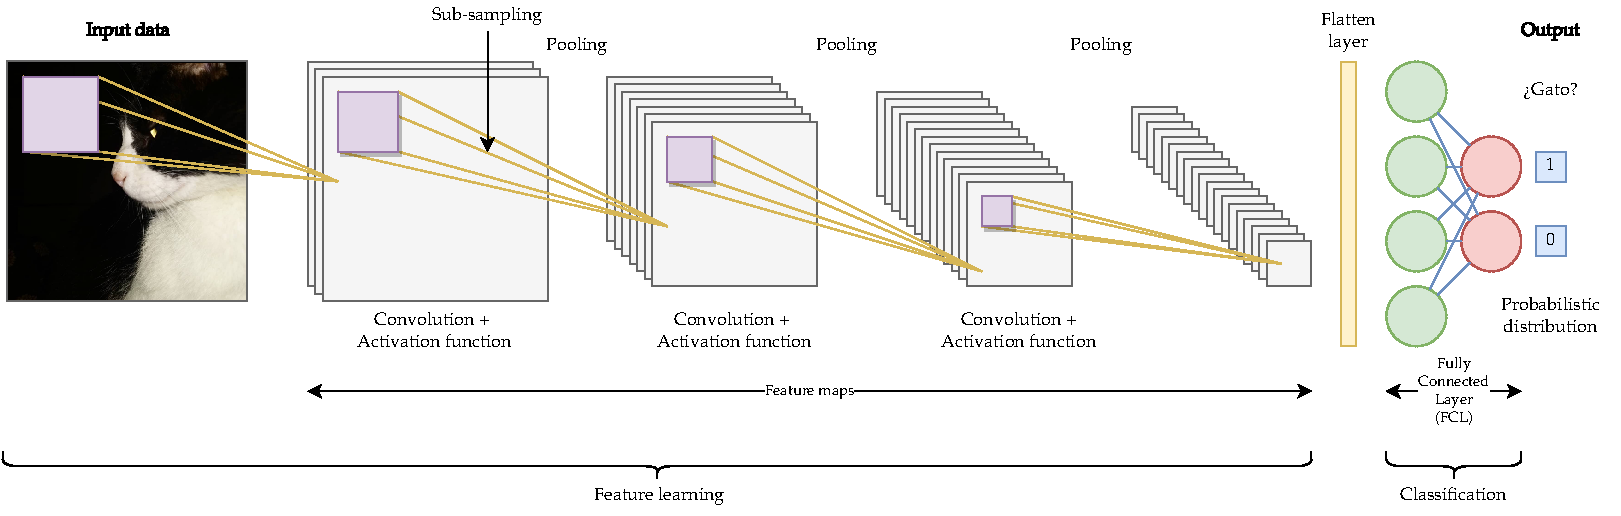
\includegraphics[width=1\textwidth]{images/cnn.pdf}
    \caption{Convolutional neural network architecture}
    \label{fig:cnn}
\end{figure}
\end{frame}

\begin{frame}
\frametitle{Generative Adversarial Networks}
\begin{figure}
    \centering
    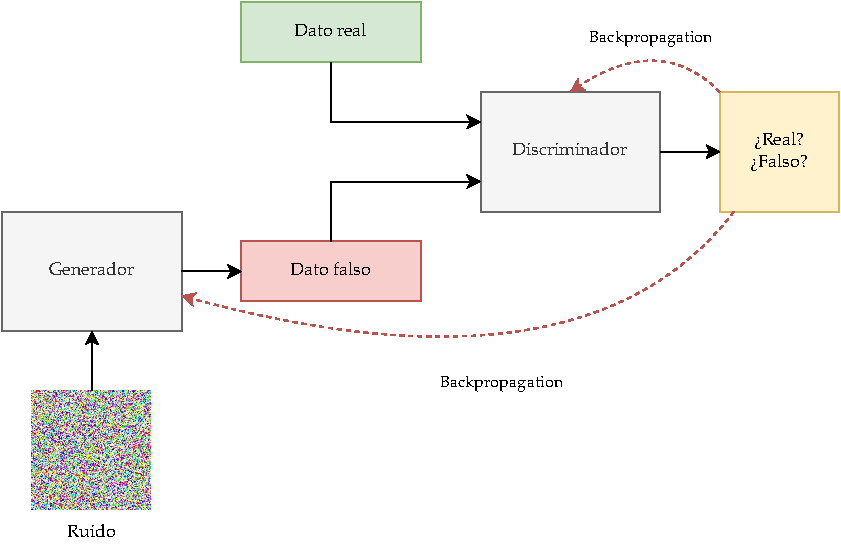
\includegraphics[width=0.8\textwidth]{images/gan.pdf}
    \caption{Generative adversarial network architecture}
    \label{fig:gan}
\end{figure}
\end{frame}

\begin{frame}
\frametitle{Geo spatial Data Types}
This is some text in the first frame. This is some text in the first frame. This is some text in the first frame.
\end{frame}

\begin{frame}
\frametitle{Vector}
Scalable data geometrically represented lines, shapes, or points.

\begin{itemize}
    \item Smaller file sizes.
    \item Better for depicting boundaries, roads and regional area.
    \item Can be styled as points, polygon color, line weights.
\end{itemize}

\begin{figure}
    \centering
    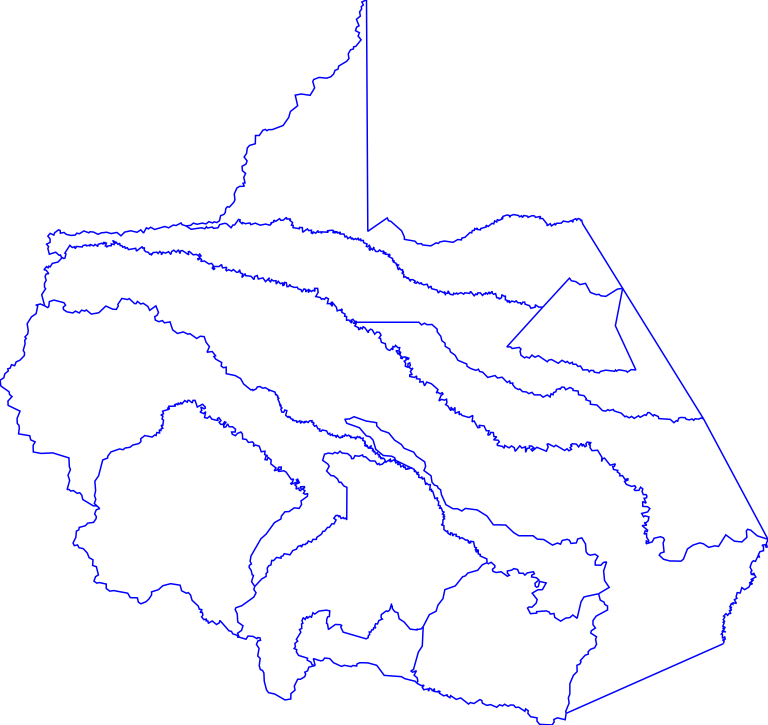
\includegraphics[width=0.35\textwidth]{images/vector.png}
    \caption{Example of vector data}
    \label{fig:vector}
\end{figure}

\end{frame}

\begin{frame}
\frametitle{Raster}

Data recorded as a pixel/grid units with image or information.

\begin{itemize}
    \item Resolution is the pixel size.
    \item Can display satellite and other photographic information.
\end{itemize}

\begin{figure}
    \centering
    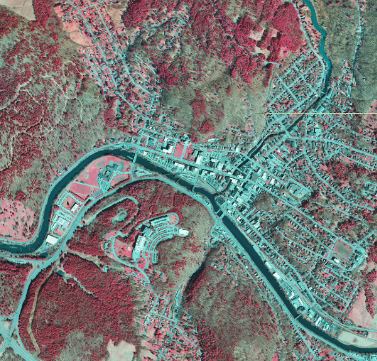
\includegraphics[width=0.35\textwidth]{images/raster.png}
    \caption{Example of raster data}
    \label{fig:raster}
\end{figure}

\end{frame}

\begin{frame}
\frametitle{Differences between vector and raster data}


\begin{figure}
    \centering
    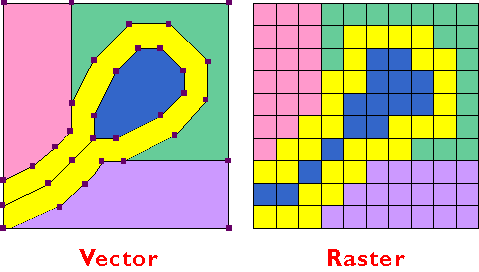
\includegraphics[width=0.5\textwidth]{images/vector_raster.png}
    \caption{Differences between vector and raster data}
    \label{fig:differences_vector_raster}
\end{figure}

Common file extensions:

\begin{itemize}
    \item Vector data: ESRI Shapefile, GEOJSON, KML/KMZ.
    \item Raster data: TIFF, JP2.
\end{itemize}

\end{frame}

\end{document}
